% -*- TeX -*-
\documentclass[aspectratio=169]{beamer}

\usepackage{listings}
\usepackage{amsmath}
\usepackage{tikz}
\usetikzlibrary{shapes,calc}

\title{Crustal Deformation Modeling Tutorial}
\subtitle{Meshing with Basic Two-Dimensional Geometry}
\author{Charles Williams \\
  Brad Aagaard \\
  Matthew Knepley}
\institute{
\includegraphics[scale=0.4]{../../logos/cig_blackfg}}
\date{June 10, 2019}


% ---------------------------------------------------- CUSTOMIZATION
\renewcommand{\thispdfpagelabel}[1]{}
\usetheme{CIG}
% Style information for PyLith presentations.

% Colors
\definecolor{ltorange}{rgb}{1.0, 0.74, 0.41} % 255/188/105
\definecolor{orange}{rgb}{0.96, 0.50, 0.0} % 246/127/0

\definecolor{ltred}{rgb}{1.0, 0.25, 0.25} % 255/64/64
\definecolor{red}{rgb}{0.79, 0.00, 0.01} % 201/0/3

\definecolor{ltpurple}{rgb}{0.81, 0.57, 1.00} % 206/145/255
\definecolor{purple}{rgb}{0.38, 0.00, 0.68} % 97/1/175

\definecolor{ltblue}{rgb}{0.2, 0.73, 1.0} % 51/187/255
\definecolor{mdblue}{rgb}{0.28, 0.50, 0.80} % 72/128/205
\definecolor{blue}{rgb}{0.12, 0.43, 0.59} % 30/110/150

\definecolor{ltltgreen}{rgb}{0.7, 1.00, 0.7} % 96/204/14
\definecolor{ltgreen}{rgb}{0.37, 0.80, 0.05} % 96/204/14
\definecolor{green}{rgb}{0.23, 0.49, 0.03} % 59/125/8
  
\definecolor{dkslate}{rgb}{0.18, 0.21, 0.28} % 47/53/72
\definecolor{mdslate}{rgb}{0.45, 0.50, 0.68} % 114/127/173
\definecolor{ltslate}{rgb}{0.85, 0.88, 0.95} % 216/225/229


\newcommand{\includefigure}[2][]{{\centering\includegraphics[#1]{#2}\par}}
\newcommand{\highlight}[1]{{\bf\usebeamercolor[fg]{structure}#1}}
\newcommand{\important}[1]{{\color{red}#1}}
\newcommand{\issue}[2]{\item[Issue:] {\color{red}#1}\\{\item[Soln:] \color{blue}#2}\\[4pt]}

\setbeamercolor{alerted text}{fg=ltgreen}
\setbeamertemplate{description item}[align left]


\newcommand{\lhs}[1]{{\color{blue}#1}}
\newcommand{\rhs}[1]{{\color{red}#1}}
\newcommand{\annotateL}[2]{%
  {\color{blue}\underbrace{\color{blue}#1}_{\color{blue}\mathclap{#2}}}}
\newcommand{\annotateR}[2]{%
  {\color{red}\underbrace{\color{red}#1}_{\color{red}\mathclap{#2}}}}
\newcommand{\eqnannotate}[2]{%
  {\color{blue}%
  \underbrace{\color{black}#1}_{\color{blue}\mathclap{#2}}}}

\newcommand{\trialvec}[1][]{{\vec{\psi}_\mathit{trial}^{#1}}}
\newcommand{\trialscalar}[1][]{{\psi_\mathit{trial}^{#1}}}
\newcommand{\basisvec}[1][]{{\vec{\psi}_\mathit{basis}^{#1}}}
\newcommand{\basisscalar}[1][]{{\psi_\mathit{basis}^{#1}}}

\newcommand{\tensor}[1]{\bm{#1}}
\DeclareMathOperator{\Tr}{Tr}

\usefonttheme[onlymath]{serif}

% minted shortcuts
\newminted{cfg}{bgcolor=ltslate,autogobble,fontsize=\tiny}
\newminted{bash}{bgcolor=ltltgreen,autogobble,fontsize=\tiny}

% PyLith components
\newcommand{\pylith}[1]{{\ttfamily\color{magenta}#1}}



% --------------------------------------------------------- DOCUMENT
\begin{document}

% ------------------------------------------------------------ SLIDE
\maketitle

% ========================================================== SECTION
\section{Meshing}
\subsection{General steps}

% ------------------------------------------------------------- LOGO
\logo{
\includegraphics[height=4.5ex]{../../logos/cig_blackfg}}

% ------------------------------------------------------------ SLIDE
\begin{frame}
  \frametitle{Meshing with Basic Two-Dimensional Geometry}
  \summary{Steps in creating a mesh}
  
  \begin{itemize}
  \item Determine geometric features needed
    \begin{itemize}
    \item Fault geometry
    \item Topography
    \item Sharp structural boundaries
    \item Magma sources with complex geometry
    \end{itemize}
  \item Create spline curve (2D) or NURBS surface (3D) in CUBIT/Trelis
  \item If using surface in several models export it for future use
  \item Use surfaces within CUBIT/Trelis to webcut or split
    volumes/surfaces
  \item Choose discretization according to type of problem
  \end{itemize}

\end{frame}

% ========================================================== SECTION
\subsection{2-D Thrust Fault Meshing Example}

% ------------------------------------------------------------ SLIDE
\begin{frame}
  \frametitle{Meshing of a thrust fault with splay}
  \summary{2-D coarse meshing of a planar thrust fault with a simulated splay fault}
  
  \begin{itemize}
  \item Two-dimensional reverse fault example\\
    \important{{\tt examples/2d/reverse}}
    \begin{itemize}
    \item All other journal files are called from either
      \important{\tt mesh\_tri.jou} or \important{\tt
        mesh\_quad\_tri.jou} using Cubit or Trelis.
      \begin{itemize}
      \item Generate basic geometry using \important{\tt
          geometry.jou}.
      \item Define mesh sizing information using \important{\tt
          gradient.jou}
      \item Define blocks and boundaries using \important{\tt
          createbc.jou}
      \end{itemize}
    \end{itemize}
  \end{itemize}


\end{frame}


% ========================================================== SECTION
\subsection{Problem geometry}

% ------------------------------------------------------------ SLIDE
\begin{frame}
  \frametitle{Meshing of a thrust fault with splay}
  \summary{Geometry with thrust (extended) and splay fault}
 
  \vfill
  \begin{center}
    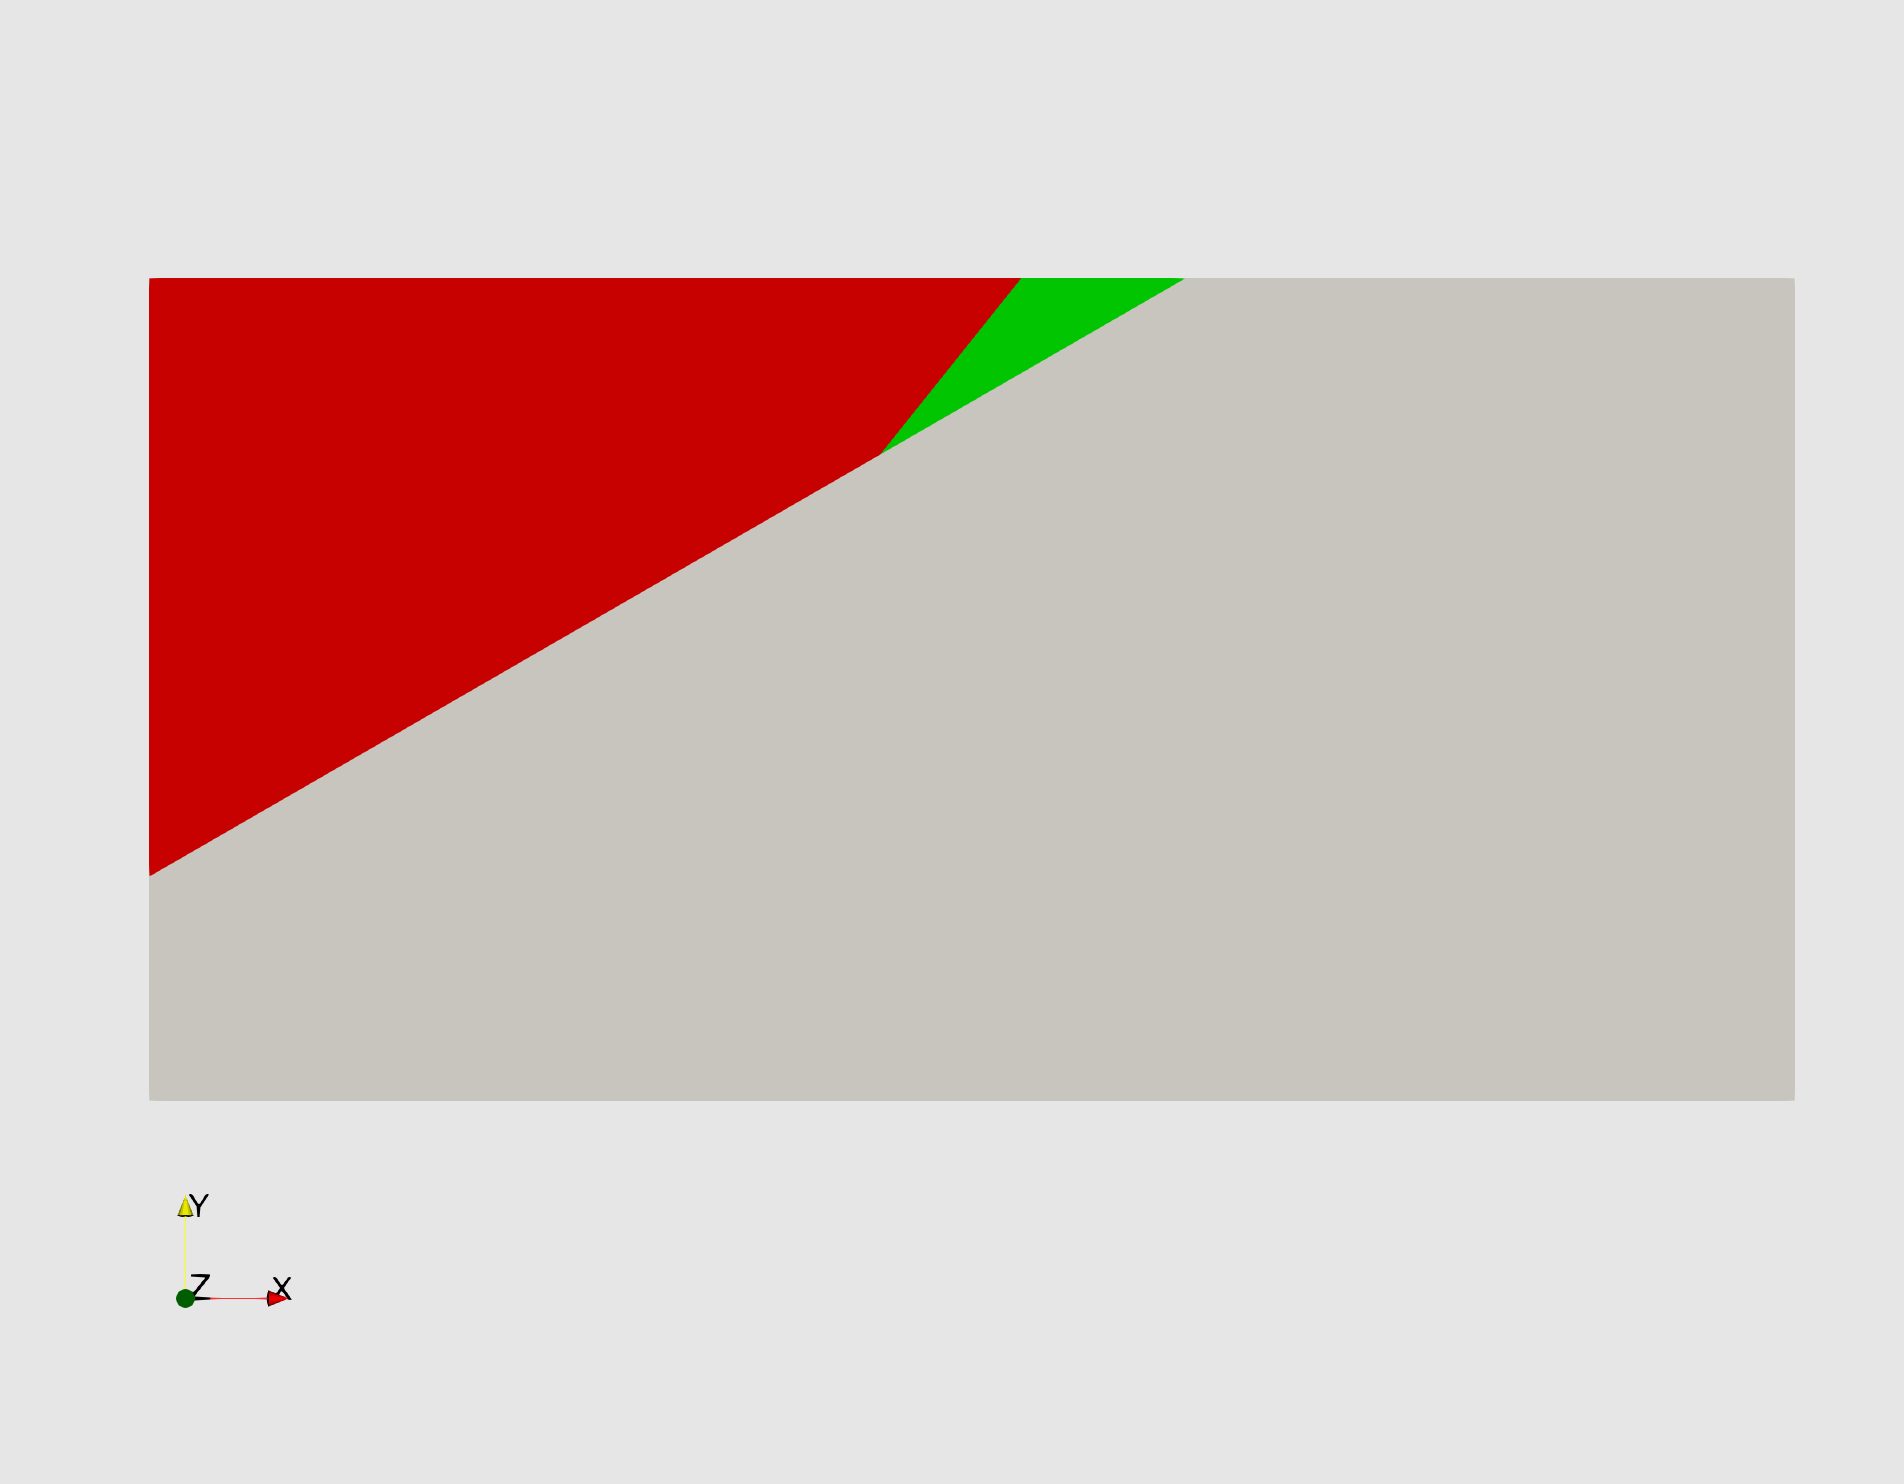
\includegraphics[height=6.1cm]{figs/reverse_geometry}
  \end{center}
  \vfill

\end{frame}


% ========================================================== SECTION
\subsection{Triangular mesh}

% ------------------------------------------------------------ SLIDE
\begin{frame}
  \frametitle{Triangular mesh generated for 2-D reverse fault example}
  \summary{Graded mesh with approximately 2.7k cells}
 
  \vfill
  \begin{center}
    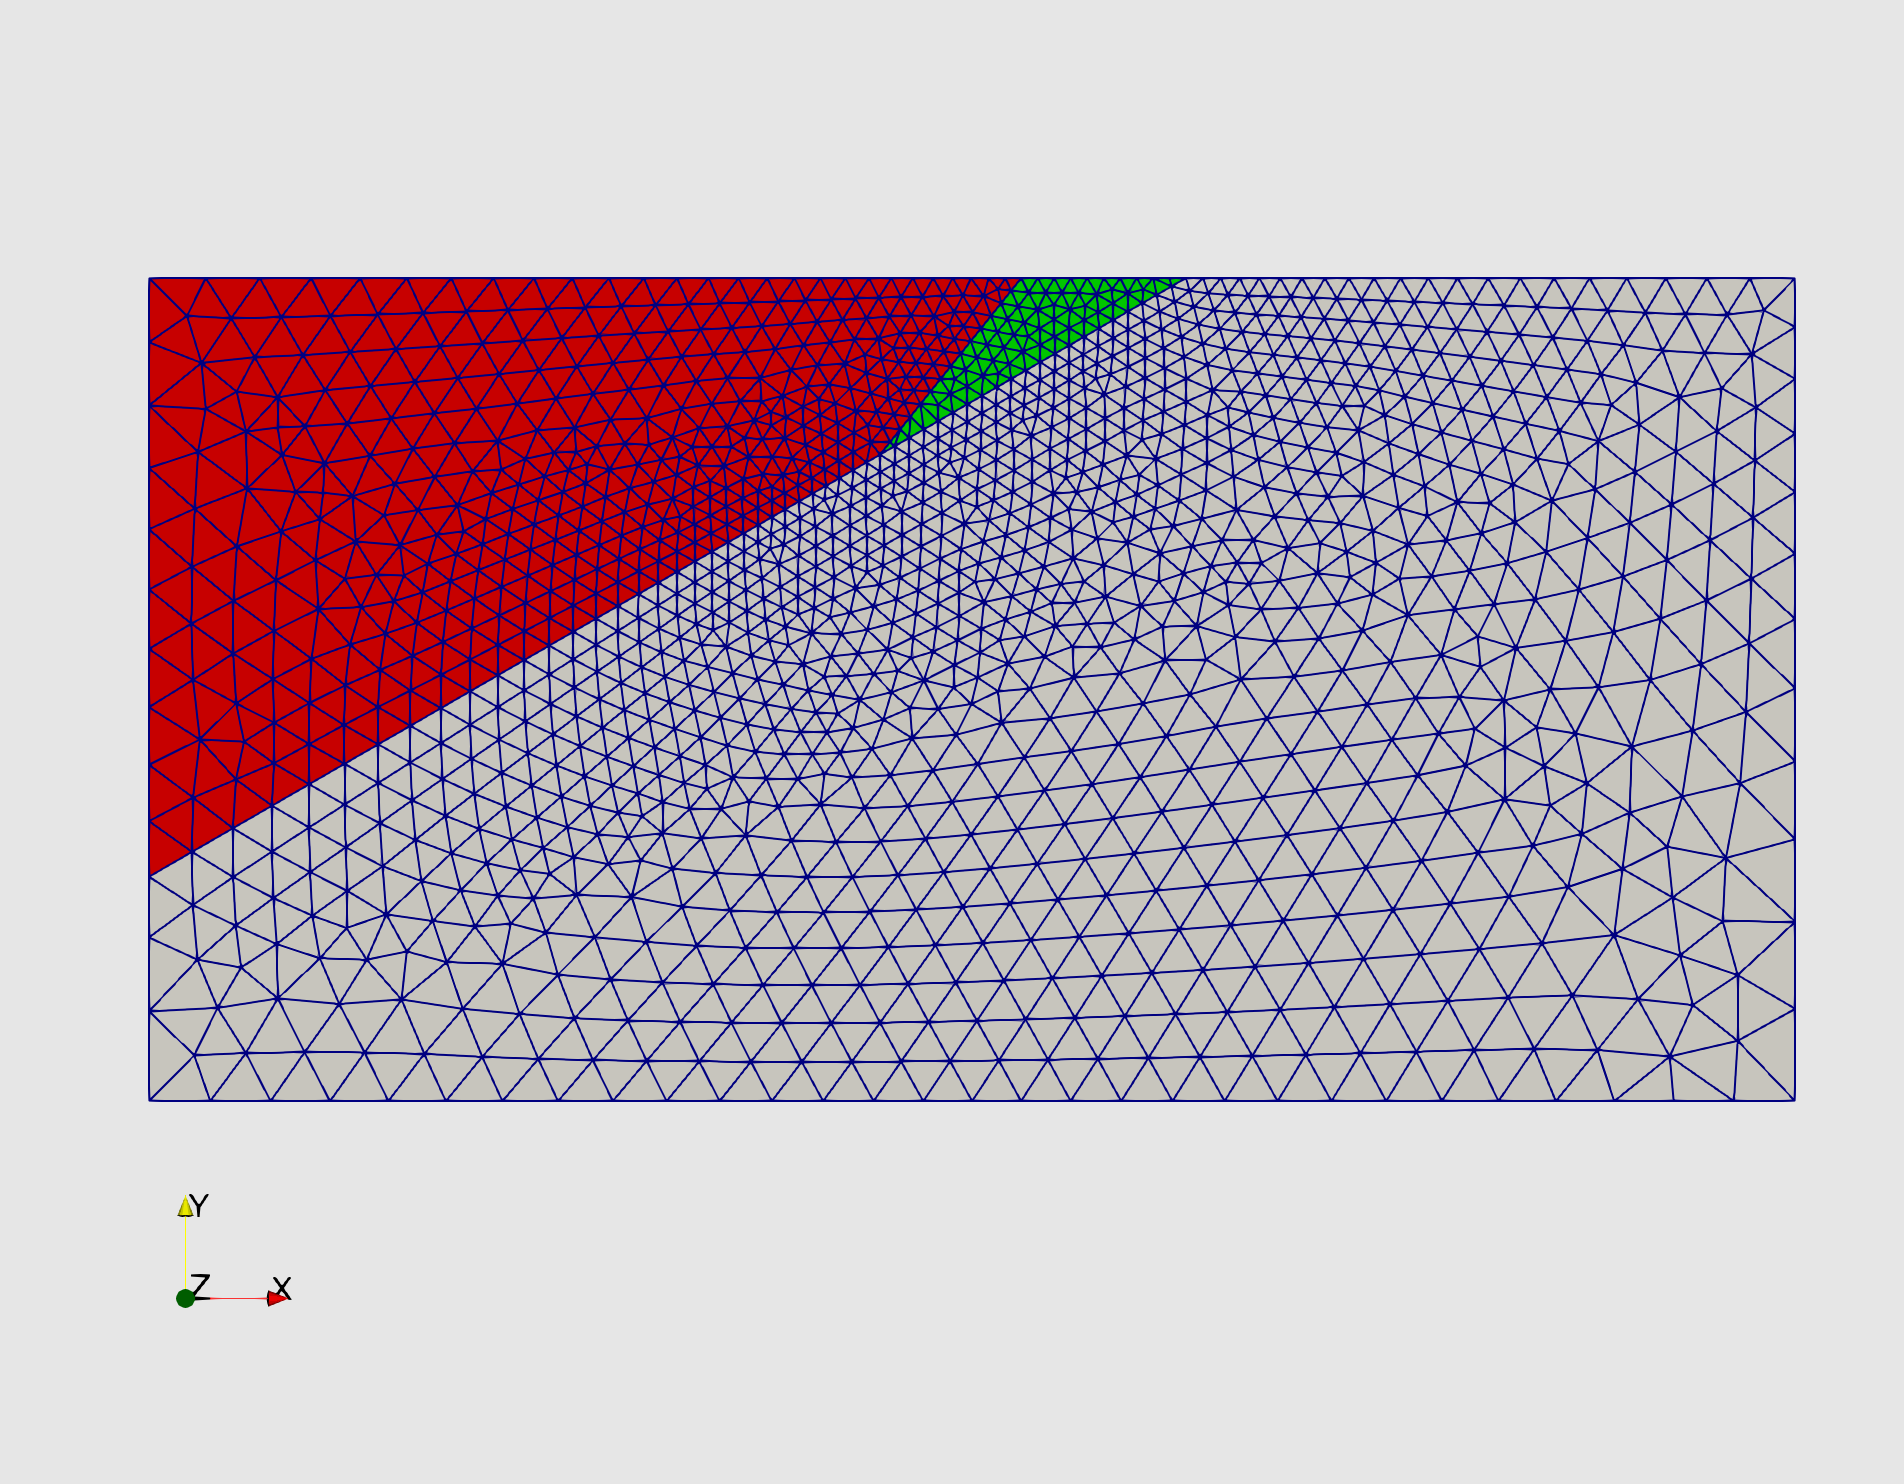
\includegraphics[height=6.1cm]{figs/reverse_trimesh}
  \end{center}
  \vfill
 
\end{frame}


% ------------------------------------------------------------ SLIDE
\subsection{What's missing}

\begin{frame}
  \frametitle{What's missing}
  \summary{Additional modifications for real problems}
  
  \begin{itemize}
  \item Mesh needs to be larger to move boundaries away from region of
    interest. One option would be to enclose this mesh in a larger
    box.
  \item The mesh is too coarse.
  \item Structural features such as the crust and slab could be added.
  \item Real faults are more likely to be curved than planar.
  \end{itemize}

\end{frame}



% ======================================================================
\end{document}


% End of file
